%!TEX root = ../main.tex 
\section{{\FEWA} and {\RAW}: Two adaptive window algorithms}
\label{sec:algo}
%
\subsection{Towards adaptive windows}
Since the expected rewards $\mu_i$ change from one pull to another, the main difficulty in the rested rotting bandits is that we cannot rely on all samples observed until time~$t$ to predict which arm is likely to return the highest reward in the future. In fact, the older a sample, the less representative it is for future rewards. This suggests constructing estimates using more recent samples. Nonetheless, discarding older rewards reduces the number of samples used in the estimates, thus increasing their variance.

In Figure~\ref{fig:SWA1}, we showed different setups in which the regret of \wSWA scales either with $\cO\pa{KLh}$ (for large $L$) or with $\tcO\pa{\nicefrac{T\sigma}{\sqrt{h}}}$ (for small $L$). \wSWA chooses a window $h$ which balances between these two costs. Yet, the two situations are quite different. In Figure~\ref{fig: adaptive_window}, we show three different reward functions with the associated data. The first one has a large decay $L> \sigma$ at the end of the sequence. The second one has a rather small decay in the middle. The last one is stationary. For these three arms, we should probably not use the same window to estimate the three values.

\begin{figure*}[h]
\centering
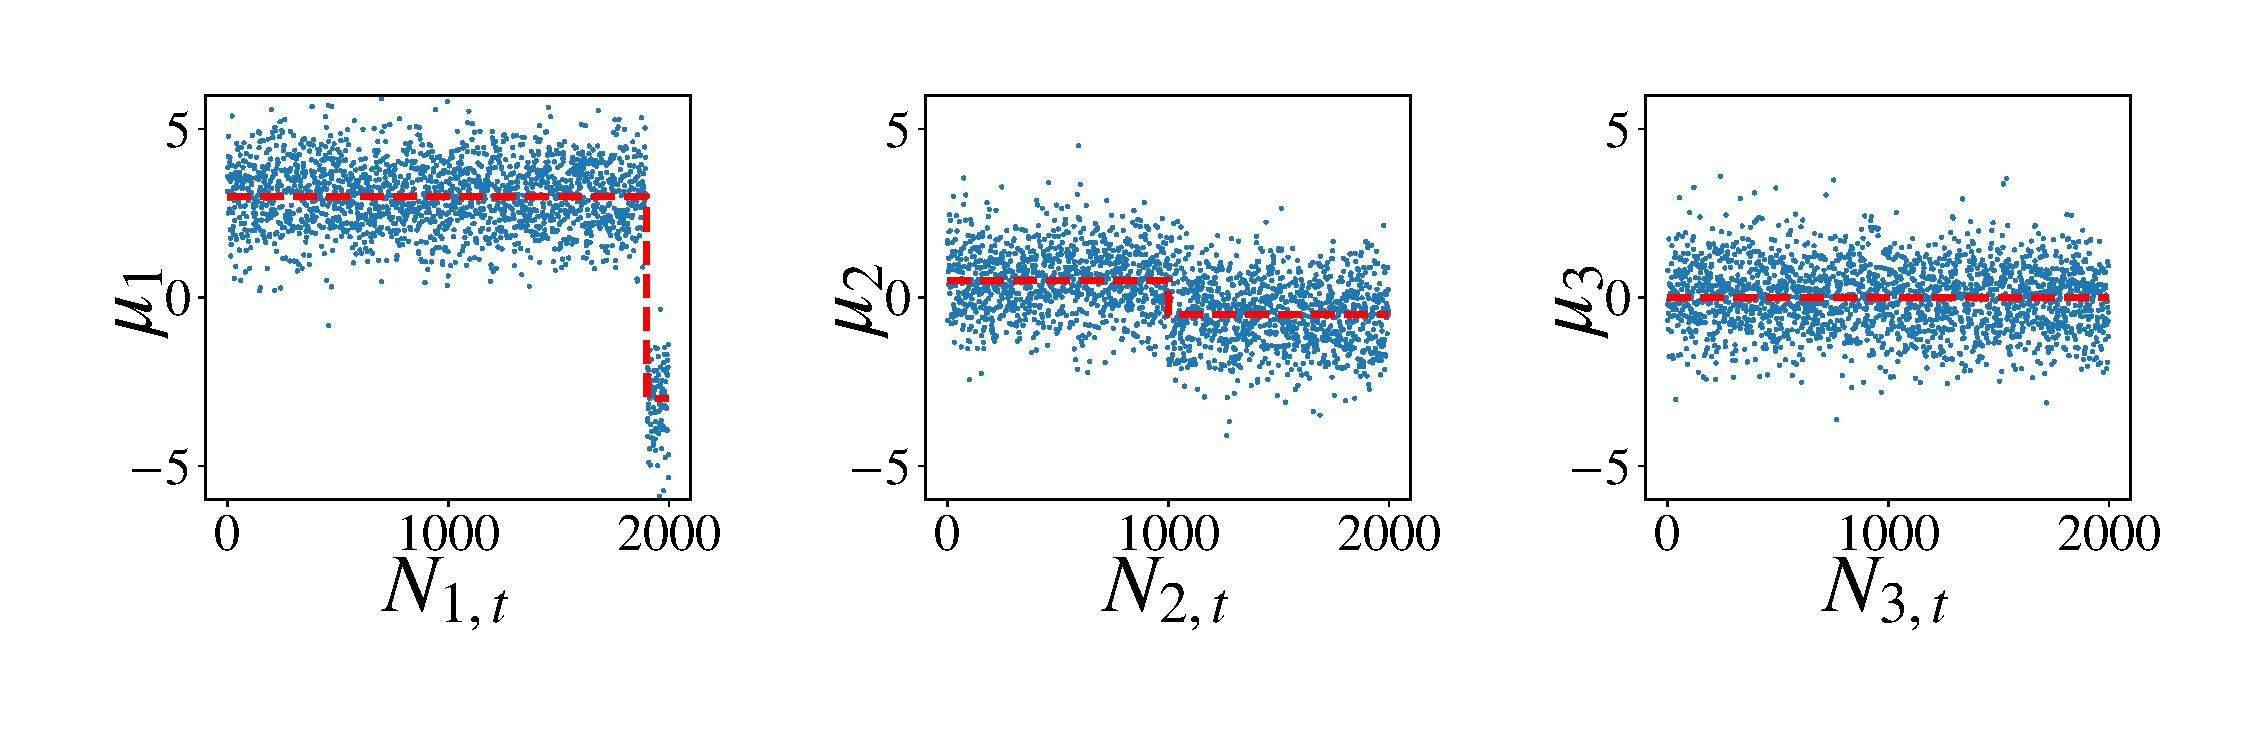
\includegraphics[clip, width= 0.99\textwidth, trim={ 1cm 2cm 1cm 1cm}]{3Rested/fig/adaptive_windows.pdf}
\caption{Three rotting reward functions (red dash line) and associated reward samples: Why should we use a single fixed window size to compare these three arms?}
\label{fig: adaptive_window}
\end{figure*}




\paragraph{A favorable event for adaptive windows}
\begin{proposition}
\label{prop:prb_favorable_event}
For any round $t$ and confidence $\delta_{t} \triangleq 2t^{-\alpha}$, let 
%
\begin{equation}
\!\HPevent\! \triangleq\! \Big\{ \forall i\!\in\!\arms,\ \forall n \!\leq\! t\!-\!1 ,\ \forall h \!\leq\! n, \big| \hmu^h_i(t, \pi) - \bmu^h_i(t,\pi) \big| \!\leq\! c(h, \delta_{t}) \!\Big\}
\label{eq:def_favorable_event}
\end{equation}
 be the event under which the estimates at a round $t$  are all accurate up to $c(h,\delta_{t}) \triangleq \sqrt{2 \subgaussian^2\log(2/\delta_t)/h}$. Then, for a policy $\pi$ which pulls each arms once at the beginning, and for all $t>K$,
\[
\PPempty\Big[\bar{\HPevent}\Big] \leq \frac{Kt^2\delta_{t}}{2}=Kt^{2-\alpha}\,.
\]
\end{proposition} 

\begin{proof}
We want to upper bound the probability
\[
\PP{\bar{\HPevent}} = \PP{\exists i \in K,\,\exists n \leq t-1, \exists h \leq\, n, \big|\hmu^h_i(n)-\bmu^h_i(n)\big|>c(h,\delta_t) }.
\]

Following the same argument as in Proposition~\ref{prop:prb_favorable_event_SWA}, there exists a sequence of random independent variable $(\epsilon'_l)_{l\in\NN}$ , $\sigma^2$ sub-Gaussian such that for $\hepsilon^h_n \triangleq (1/h) \sum_{l=n-h+1}^n \epsilon'_l$ we get, 
\begin{align*}
    \PPv\Big[\exists n \leq t-1, \exists h &\leq\, n, \big|\hmu^h_i(t-1,\pi)-\bmu^h_i(t-1,\pi)\big|>c(h,\delta_t) \Big]\\
    &= \PP{\,\exists n \leq t-1, \exists h \leq n,\, |\hepsilon^h_n|>c(h,\delta_t) }\\
    &\leq \sum_{n=1}^{t-1}\sum_{h=1}^n \PP{|\hepsilon^h_n|>c(h,\delta_t)} \\
    &\leq  \frac{t(t-1)}{2}\cdot \delta_t \,,
\end{align*}
where we used the Chernoff inequality in the last line. Thus, a union bound  over the arms allows us to conclude that
\[
\PPempty \Big[\bar{\HPevent}\Big]\leq \frac{K \delta_t t^2}{2}\cdot
\]
\end{proof}
\begin{remark}
Compared to the unique favorable event we used for \SWA (see Equation~\ref{eq:def_favorable_event_SWA}), we use a favorable event for each round $t$. It will be helpful to obtain anytime guarantees for our algorithms. Moreover, $\HPevent$ control the deviation of any statistic $\hmu_i^h(n)$ for any possible $h$, $i$ and $n$. This is different from $\HPSWA$ which uses a fixed $h$. 
\end{remark}

\subsection{{\FEWA}: Filtering on expanding window average}
\label{ss:fewa}
In Alg.\,\ref{alg:FEWA}, we introduce \FEWA (or~$\piF$) that at each round $t$, relies on estimates using windows of increasing length to filter out arms that are sub-optimal with high probability and then pulls the least pulled arm among the remaining arms. 
 \begin{figure*}[!ht]
 \begin{minipage}{\textwidth}
\renewcommand*\footnoterule{}
\begin{savenotes}
\begin{algorithm}[H]
\caption{\FEWA}
\label{alg:FEWA}
\begin{algorithmic}[1]
\Require $\arms$,  $\subgaussian$, $\alpha$
\For{$t \gets 1, 2, \dots, K \do $}{\footnotesize \Comment{\emph{Pull each arm once}}}
	\State \textsc{Pull}  $i_t \gets t$; \textsc{Receive} $o_{t}$
	\State $N_{i_t} \gets 1$
	\State $\left\{\hmu_{i_t}^h\right\}_h \gets \UPDATE(\left\{\hmu_{i_t}^h\right\}_h, o_t)$\label{algline:fewa-update1}
\EndFor
\For{$t \gets K+1, K+2, \dots \do $}
	\State $h\leftarrow 1$ 
	{\footnotesize \Comment{\emph{initialize bandwidth}}}
	\State $\arms_1 \leftarrow \arms$ 
	{\footnotesize \Comment{\emph{initialize with all the arms}}}
	\State $i_t \gets {\tt none}$
	\While{$i_t$ is  ${\tt none}$} \label{algline:fewa-while}
		\State $\arms_{h+1} \leftarrow {\FILTER}(\arms_{h} ,h, \alpha, \sigma)$ \label{algline:fewa-filter}
		\State $h \leftarrow h + 1$ \label{algline:fewa-window}
		\If{$\exists i \in \arms_{h}$ such that $N_{i_t}=h$}
			\label{algline:fewa-condition}
			\State \textsc{Pull}  $i_t \in \left\{ i \in \arms_h | N_{i_t} = h \right\}$\footnote{One can choose the tie break selection rule arbitrarily, e.g. by selecting the arm with the smallest index.}; \textsc{Receive} $o_{t}$\label{algline:fewa-pull}
		\EndIf
	\EndWhile
    \State $N_{i_t} \leftarrow N_{i_t} +1$
	\State $\left\{\hmu_{i_t}^h\right\}_h \gets \UPDATE(\left\{\hmu_{i_t}^h\right\}_h, o_t)$\label{algline:fewa-update2}
\EndFor
\end{algorithmic}
\end{algorithm}
\end{savenotes}
\end{minipage}
\end{figure*}

We first describe the subroutine {\FILTER} in Alg.\,\ref{alg:filter}, which receives a set of active arms $\arms_h$, a window~$h$, a confidence bound tuning parameter $\alpha$ and the subgaussian parameter $\sigma$  as input and returns an updated set of arms $\arms_{h+1}$. For each arm~$i \in \arms_h$ (that has all been pulled~$n \geq h$ times), the algorithm has stored an estimate $\hmu_i^h$ that averages the $h$ most recent rewards observed from~$i$. 
The subroutine \FILTER discards all the arms whose mean estimate (built with window~$h$) from $\arms_h$  is lower than the empirically best arm by more than twice a threshold $c(h, \delta_t)$ constructed by standard Hoeffding's concentration inequality (see Prop.\,\ref{prop:prb_favorable_event}).



\begin{algorithm}[!ht]
\caption{{\FILTER}}
\label{alg:filter}
\begin{algorithmic}[1]
\Require $\arms_{h}$, $h$, $\alpha$, $\sigma$
\State $c(h, \delta_t) \leftarrow \sqrt{2\alpha\sigma^2\log{(t)}/h }$
\State $\hmu^h_{\max}  \leftarrow \max_{i \in \arms_{h}}\hmu_i^h$\label{algline:filter-max}
\For{$ i \in \arms_{h}$}
	\State $\Delta_i \leftarrow  \hmu^h_{\max} - \hmu^h_{i} $ \label{algline:filter-delta}
	\If{$\Delta_i \leq 2c(h,  \delta_t) $}
	\State add $i$ to $\arms_{h+1}$ \label{algline:filter-add}
	\EndIf
\EndFor
\Ensure $\arms_{h+1}$
\end{algorithmic}
\end{algorithm}



The \FILTER subroutine is used in \FEWA to incrementally refine the set of active arms, starting with a window of size $1$, until the condition at Line~\ref{algline:fewa-condition} is met. As a result, $\arms_{h+1}$ only contains arms that passed the filter for all windows from $1$ up to $h$. Notice that it is important to start filtering arms from a small window and to keep refining the previous set of active arms. 
In fact, the estimates constructed using a small window use recent rewards, which are closer to the future value of an arm. As a result, if there is enough evidence that an arm is suboptimal already at a small window $h$, it should be directly discarded. On the other hand, a sub-optimal arm may pass the filter for small windows as the threshold $c(h , \delta_t)$ is large for small $h$ (i.e., because a few samples are used in constructing $\hmu_i^h$, the estimation error may be high). Thus, \FEWA keeps refining $\arms_{h}$ for larger windows in the attempt of constructing more accurate estimates and discard more sub-optimal arms. This process stops when we reach a window as large as the number of samples for at least one arm in the active set $\arms_{h}$ (i.e., Line~\ref{algline:fewa-condition}). At this point, increasing $h$ would not bring any additional evidence that could refine $\arms_{h}$ further (recall that $\hmu^h_i$ is not defined for $h > N_i$). Finally,  \FEWA selects the active arm $i_t$ whose number of samples matches the current window, i.e., the least pulled arm in $\arms_{h}$. The set of available rewards and the number of pulls are then updated accordingly. 

\paragraph{Core guarantee on the favorable event} 
We derive an important lemma that provides support for the arm selection process obtained by a series of refinements through the \FILTER subroutine. Recall that at any round $t$, after pulling arms $\{ \Nitmone\}_i$ the greedy (oracle) policy would select an arm 
%
\begin{align*}
i^\star_t \pa{\left\{ \Nitmone \right\}_i}  \in  \argmax_{i \in \arms} \mu_i \left( \Nitmone\right).
\end{align*}
%
We recall that $\mu^+_t(\piF) \triangleq \max_{i \in \arms} \mu_i (\Nitmone)$ the reward that could be obtained by pulling~$i^\star_t$ at a round $t$. 
While \FEWA cannot directly match the performance of the oracle arm, the following lemma guarantees that the past performance of the selected arm is close enough compared to the current best arm value. 

\begin{restatable}{lemma}{restalemmafewa}
\label{lem:core-FEWA}
For {\FEWA} tuned with $\alpha$, on the favorable event $\HPevent$, if an arm~$i$ passes through a filter of window $h$ at a round $t$, i.e., $i\in\ \arms_h$, then the average of its $h$ last pulls satisfies
%
\begin{equation}\label{eq:fundamental-eq-FEWA}
\bmu^{h}_i(\Nitmone ) \geq  \mu^+_t(\piF) - 4 c(h, \delta_t).
\end{equation}
Therefore, at a round $t$, on favorable event $\HPevent$, if arm~$i_{t}$ is selected by {\FEWA($\alpha$)}, for any $h \leq \Nitmone$,  the average of its $h$ last pulls cannot deviate significantly from the best available arm at that round, i.e.,
%
\begin{equation*}
\bar{\mu}^{h}_{i_{t}}(\Nitmone) \geq \mu^+_t(\piF) - 4 c(h, \delta_{t}).
\end{equation*}
\end{restatable}

\begin{proof}
We will prove this property for a more general rotting feedback model than the rested rotting one presented in Equation~\ref{eq:rested-feedback}. If arm $i$ is selected at the round $t$, the learner $\pi$ receives,
\[
o_t \triangleq \mu_{i, \, t} + \noise_t  \;\; \text{with}\; \EE{ \noise_t | \historyt }= 0 \;\; \text{and} \; \forall \lambda \in \R, \; \EE{ e^{\lambda\noise_t}} \leq e^{\frac{\subgaussian\lambda^2}{2}},
\]
with $\left\{ \mu_{i, \, t}\right\}_{t\leq T}$ a non-increasing sequence. We do not specify how the reward is rotting, while it was assumed in Equation~\ref{eq:rested-feedback} that the reward function was evolving with the number of pull $\Nitmone$ of arm $i$ at the round $t$. With this reward model, we cannot use $\bmu^{h}_{i}(\Nitmone^{\pi})$ to refer to $\bmu_i^h(t,\pi)$, the average of the $h$ last means associated to arm $i$ (see the definition in Equation~\ref{eq:def-bmu} and the following remark). We will use this more general proof in the next Chapter~\ref{ch:restless}.

Let $i \in \arms_h$ be an arm that passed a filter of window $h$ at the round $t$.
First, we use the confidence bound for the estimates and we pay the cost of keeping all the arms up to a distance $2c(h,  \delta_t)$ of $\hmu^{h}_{\max,\, t} \triangleq \max_{j \in \arms_h} \hmu_i^h(t,\piF)$,
\begin{equation}
\label{1}
\bmu_i^h(t,\piF)\geq \hmu_i^h(t,\piF)- c(h,  \delta_t) \geq \hmu^h_{\max,t} - 3c(h, \delta_t)
\geq \max_{j \in \arms_h}\bmu_j^h(t,\piF)  - 4 c(h, \delta_t),
\end{equation}
where in the last inequality, we used that for all $j \in \arms_h,$ \[\hmu^{h}_{\max,t} \geq  \hmu_j^h(t,\piF)  \geq \bmu_j^h(t,\piF)  - c(h, \delta_t).\]
Second, we call $t_{i,t} < t$ the last round at which arm $i$ was selected. Since the means of arms are decaying, we know that 
\begin{align}
\label{2}
 \mu^+_t(\piF) &\triangleq \mu_{i^\star_t, \, t} \nonumber\\
 &\leq  \mu_{i^\star_t, \, t_{i,t}} =  \bmu_i^1(t,\piF)  \nonumber\\
 &\leq \max_{j \in \arms}\bmu_j^1(t,\piF)  = \max_{j \in \arms_1} \bmu_j^1(t,\piF).
\end{align}
Third, we show that the largest average of the last $h'$ means of arms in $\arms_{h'}$ is increasing with~$h'$,
\begin{equation*}
\forall  h' \leq h ,  \max_{j \in \arms_{h'+1}}\bmu_j^{h'+1}(t,\piF)   \geq \max_{j \in \arms_{h'}}\bmu_j^{h'}(t,\piF). 
\end{equation*}
To show the above property, we remark that thanks to our selection rule, the arm that has the largest average of means, always passes the filter. Formally, we show that $\argmax_{j \in \arms_{h'}}\bmu_j^{h'}(t,\piF) \subseteq \arms_{h'+1}.$ 
Let $i^{h'}_{\max} \in \argmax_{j \in \arms_{h'}}\bmu_j^{h'}(t,\piF)$. Then, for such $i^{h'}_{\max}$, we have
\begin{equation*}
\hmu_{i^{h'}_{\max}}^{h'}(t,\piF) \geq \bmu_{i^{h'}_{\max}}^{h'}(t,\piF) - c(h', \delta_t) 
\geq \bmu^{h'}_{\max,t} - c(h', \delta_t) \geq \hmu^{h'}_{\max,t}- 2c(h', \delta_t),
\end{equation*}
where the first and the third inequality are due to concentration of the estimates on $\HPevent$, while the second one is due to the definition of $i^{h'}_{\max}$. 

Since the arms are decaying, the average of the last $h' +1$ mean values for a given arm is always greater than the average of the last $h'$ mean values
and therefore, 
\begin{equation}
\label{3}
 \max_{j \in \arms_{h'}}\bmu_j^{h'}(t,\piF) =   \bmu_{i^{h'}_{\max}}^{h'}(t,\piF) \leq \bmu_{i^{h'}_{\max}}^{h'+1}(t,\piF) \leq \max_{j \in \arms_{h'+1}}\bmu^{h' +1 }_{j}(t,\piF), 
\end{equation}
because $i^{h'}_{\rm max} \in \arms_{h'+1}$. Gathering Equations~\ref{1}, \ref{2}, and~\ref{3} leads to the first claim of the lemma,
\begin{align*}
\bmu^{h}_i(t,\piF)
&\stackrel{\eqref{1}}{\geq} \max_{j \in \arms_h}\bmu^{h}_{j}(t,\piF) - 4c(h, \delta_t)\\
&\stackrel{\eqref{3}}{\geq} \max_{j \in \arms_1}\bmu^{1}_{j}(t,\piF)- 4c(h,  \delta_t)\\
&\stackrel{\eqref{2}}{\geq}  \mu^+_t(\piF) - 4c(h, \delta_t).
\end{align*}
To conclude, we remark that if $i$ is pulled at the round $t$, then by the condition at Line~\ref{algline:fewa-condition} of Algorithm~\ref{alg:FEWA}, it means that $i$ passes through all the filters from $h=1$ up to $\Nitmone$. Therefore, for all $h\leq \Nitmone$,
%
\begin{equation}
\bmu^{h}_i(t,\piF) \geq  \mu^+_t(\piF) - 4 c(h, \delta_t).
\end{equation}
\end{proof}

\subsection{{\RUCB}: Rotting Adaptive Window Upper Confidence Bound}
\label{ss:rawucb}

 \begin{minipage}{\textwidth}
\renewcommand*\footnoterule{}
\begin{savenotes}
\begin{algorithm}[H]
\caption{\RUCB}
\label{alg:RAWUCB}
\begin{algorithmic}[1]
\Require $\arms$,  $\subgaussian$, $\alpha$
\For{$t \gets 1, 2, \dots, K \do $}{\footnotesize \Comment{\emph{Pull each arm once}}}
	\State \textsc{Pull}  $i_t \gets t$; \textsc{Receive} $o_{t}$
	\State $N_{i_t} \gets 1$
	\State $\left\{\hmu_{i_t}^h\right\}_h \gets \UPDATE(\left\{\hmu_{i_t}^h\right\}_h, o_t)$ \label{algline:raw-update1}
\EndFor
\For{$t \gets K+1, K+2, \dots \do $}
	\State \textsc{Pull}  $i_t \in \argmax_i \min_{h \leq N_{i}}\pa{\hmu_i^h + c(h, \delta_t)} $\footnote{One can choose the tie break selection rule arbitrarily, e.g. by selecting the arm with the smallest index.}; \textsc{Receive} $o_{t}${\footnotesize \Comment{\emph{cf.\,\eqref{eq:raw_index}}}}; \label{algline:raw-pull}
	\State  $N_{i_t} \gets N_{i_t} +1$
	\State $\left\{\hmu_{i_t}^h\right\}_h \gets \UPDATE(\left\{\hmu_{i_t}^h\right\}_h, o_t)$\label{algline:raw-update2}
\EndFor
\end{algorithmic}
\end{algorithm}
\end{savenotes}
\end{minipage}



We will study a single class of policies which select at each round $t$ the arm with the maximal index of the form
\begin{align}
\label{eq:raw_index}
\operatorname{ind}(i,t, \delta_{t}) \triangleq \min_{h\leq N_{i,t-1}}\pa{ {\hmu}_i^h(\Nitmone) + c(h,\delta_{t})}\quad \text{ with } \; \delta_{t} \triangleq \frac{2}{t^\alpha} .
\end{align}
We set and call this algorithm Rotting Adaptive Window UCB (\RUCB). There is a bias-variance trade-off for the window choice: more variance for smaller sizes of the window $h$ and more bias for larger $h$. The goal of \RUCB is to adaptively select the right window to compute the tightest UCB. \RUCB uses the indexes of \UCBone computed on all the slices of each arm's history which include the last pull. When the rewards are rotting, all these indexes are upper confidence bounds on the \textit{next value}.  Thus, \RUCB simply selects the tightest (minimum) one as the index of the arm: it is a pure UCB-index algorithm. By contrast, when the reward can increase, the learner can only derive upper-confidence bound on past values which are loosely related to the next value. Hence, all the UCB-index algorithms in the restless non-stationary literature need to add change-detection sub-routine, active random exploration, or passive forgetting mechanism. 

\paragraph{Core guarantee on the favorable event}

\begin{restatable}{lemma}{restalemmaraw}
\label{lem:core-RAWUCB}
At the round $t$, on favorable event $\HPevent$, if arm~$i_{t}$ is selected by \RUCB($\alpha$), for any $h \leq N_{i,t-1}$,  the average of its $h$ last pulls cannot deviate significantly from the best available arm at that round, i.e.,
%
\begin{equation*}
\bar{\mu}_{i_t}^{h}(N_{i_t,\, t-1}) \geq \max_{i \in \arms} \mu_{i}(\Nitmone) - 2 c(h, \delta_t)\,.
\end{equation*}
\end{restatable}
This lemma is comparable with Lemma~\ref{lem:core-FEWA} about the algorithm \FEWA. Yet, \RUCB has tighter guarantees than \FEWA (2 versus 4 confidence bands), which is the benefit of upper confidence bounds index policies over confidence bound filtering policies. 

\begin{proof}
Like for Lemma~\ref{lem:core-FEWA} (see its proof), our proof is done in a more general rotting framework that can be used in the next chapter. 

We denote by $
i^\star_t \in \argmax_{i\in \possibleArms}{\mu_i(t,N_{i,t-1})}
$, a best available arm at time $t$ and 
\[
h_{i,t}^{\min} \in \argmin_{h\leq \Nitmone }{\hat{\mu}_i^h(t,\pi) + c(h,\delta_t)},
\]
a window which minimizes \RAWUCB index at time $t$ for arm $i$. Hence, because the reward functions are non-increasing, we know that 
\begin{equation*}
 \mu_{i^\star_t}(t, N_{i^\star_t,t-1}) \leq   \bar{\mu}_{i^\star_t}^1(t,\pi) \leq \cdots \leq  \bar{\mu}_{i^\star_t}^{h_{i^\star_t,t}^{\min}}(t,\pi)\cdot
\end{equation*}
On the high-probability event $\xi_t$, we know that the true average of the means cannot deviate significantly from the average of the observed quantity,
\begin{equation*}
\bar{\mu}_{i^\star_t}^{h_{i^\star_t,t}^{\min}}(t, \pi) \leq \hat{\mu}_{i^\star_t}^{h_{i^\star_t,t}^{\min}}(t,\pi) + c(h_{i^\star_t,t}^{\min},\delta_t)\,.
\end{equation*}
We know that the selected arm $i_t$ at time $t$ has the largest index, hence, 
\[
\hat{\mu}_{i^\star_t}^{h^{\min}_{i^\star_t,t}}(t, \pi) + c(h^{\min}_{i^\star_t,t},\delta_t) \leq \hat{\mu}_{i_t}^{h^{\min}_{i_t,t}}(t, \pi) + c(h^{\min}_{i_t,t},\delta_t).
\]
From $h_{i,t}^{\min}$ definition, we know that this quantity is below any upper-confidence bound for any other window $h$
\[
\hat{\mu}_{i_t}^{h^{\min}_{i_t,t}}(t, \pi) + c(h^{\min}_{i_t,t},\delta_t) \leq \hat{\mu}_{i_t}^{h}(t, \pi) + c(h,\delta_t).
\]
Finally, using again the concentration of the average on the $\HPevent$, 
\[
\hat{\mu}_{i_t}^{h}(t, \pi) + c(h,\delta_t) \leq \bar{\mu}_{i_t}^{h}(t, \pi) + 2c(h,\delta_t)\,.
\]
Hence, putting all the equations together, we can write
\begin{equation*}
\bar{\mu}_{i_t}^{h}(t, \pi) \geq \max_{i \in \possibleArms} \mu_{i}(t,N_{i,t-1}) - 2 c(\window, \delta_t).
\end{equation*}
\end{proof}